\documentclass{article}
\usepackage{graphicx} % Required for inserting images
\usepackage[natbibapa]{apacite}
\usepackage[colorlinks=true,linkcolor=black,citecolor=black,urlcolor=black]{hyperref}
\usepackage{amsmath}
\usepackage{amssymb}


\title{\vspace{-2cm}Assignment 2\\
    Bop It}

\author{Tymur Mykhalievskyi\\ 7031100\\ tymy00001@stud.uni-saarland.de}
\date{\today}


\begin{document}

\maketitle

\section{Introduction}
When one thinks about a classical machine learning task, one usually imagines a dataset with a set of features and a target variable. The goal is to learn a function that maps the features to the target variable. Typically, one would make a hypothesis about the form of the function prior to training. This approach sometimes works well, but other times it does not. In this report, we will explore a deeper approach, instead of blindly guessing the form of the function, we will try to estimate whether any function can be learned at all. 

\section{Reliable Fraction of Information}
\label{sec:rfi}
We begin with the work by \cite{mandros2017}. The authors propose a method to estimate the fraction of information between the features and the target variable. The fraction of information is a measure of the amount of information that the features provide about the target variable. The main problem with the maximum likelihood estimation of fractional information is high false positive rate, which leads to overestimation of the fraction of information. The authors propose an idea to subtract the estimated bias under the assumption of independence between the features and the target variable. Formally, the reliable fraction of information is defined as \citep{mandros2017}:
\[
\hat{F}_0(X,Y) = \hat{F}(X,Y) - \frac{\hat{\mathbb{E}}_0[\hat{I}(X,Y_\sigma)]}{\hat{H}(Y)} = \hat{F}(X,Y) - \frac{1}{\hat{H}(Y)} \cdot \frac{1}{n!}\sum_{\sigma\in S_n}\hat{I}(X,Y_\sigma)
\]
where $X, Y$ are the features and the target variable, $\hat{F}$ is the estimated fraction of information via maximum likelihood estimation, similarly to $\hat{I}$ and $\hat{H}$, which are MLE of mutual information and entropy respectively. $\hat{\mathbb{E}}_0$ represents the bias coming from the expected value under the assumption of independence between $X$ and $Y$, which is estimated by averaging over all permutations of $Y$. Correspondingly, $Y_\sigma$ is one of the permutations of $Y$ coming from the group of $n!$ bijections describing all permutations $S_n$.

Furthermore, the authors proceed to optimize the computational complexity of the estimation to make it more feasible. The resulting estimator is a biased estimator, which is consistent and converges to the true value of the fraction of information. More importantly it is way more robust to the false positive rate. However, the accounted bias is based on the expected value of the mutual information under the assumption of independence. Hence, the expectation under the null is not a strict upper bound. Therefore, it is not guaranteed that positive values of the fraction of information indicate that the features and the target variable are dependent. However, empirically it behaves way better than the naive maximum likelihood estimation of the fraction of information. 

In addition, the estimator is consistent, which means that it converges to the true value of the fraction of information as the sample size increases. Moreover, empirical evaluations show that the estimator lost only a bit of variance compared to the maximum likelihood estimation. This is a very important observation considering the bias-variance trade-off.

\section{Top-k Dependencies}
\subsection{Reliable Fraction of Information for Top-k Dependencies}
In \autoref{sec:rfi} we only partially discussed the work by \cite{mandros2017}. The second part of the paper is dedicated to the problem of finding the top-k dependencies between the features and the target variable. 

The main issue when solving this problem is difficulties in guarantees of optimality of the subset of features. More formally the problem can be formulated as follows \citep{mandros2017}:

\begin{quote}
    Given a dataset $D_n$ consisting of $n$ i.i.d. samples of random variables $\mathcal{I}$ and $Y$, and a number $k$, find a family $\mathcal{F}_k$ of variable sets 
    $\mathcal{X}_1, \ldots, \mathcal{X}_k \subseteq \mathcal{I}$ such that no variable set outside $\mathcal{F}_k$ has a higher $\hat{F}_0$-score than any of the sets in $\mathcal{F}_k$, 
    i.e., for all $\mathcal{X} \in \mathcal{F}_k$ and $\mathcal{Z} \in \mathcal{P}(\mathcal{I}) \setminus \mathcal{F}_k$ it holds that $
    \hat{F}_0(\mathcal{Z}; Y) \leq \hat{F}_0(\mathcal{X}; Y).$
\end{quote}

The authors propose a so-called Best-First Branch-and-Bound algorithm to solve this problem. The main essence is in the 
bounding function, which is used to prune the search space. It is a crucial part of the algorithm, since it gives guarantees of optimality of the found solution. Given the fact that the bound function is admissible the algorithm only prunes the search space when no optimal solution can be found in the pruned part. Hence, after visiting all nodes in the search space, the algorithm will find the optimal solution.

Another important aspect is the computational complexity of the algorithm, which according to the empirical evaluations is low on some datasets, but can be high on others. This comes from the fact that the runtime is still exponential in the worst case. However, the pruning can sometimes substantially improve the running time, pruning up to $99\%$ of the nodes in some cases. The authors also propose $\alpha$ parameter to control the trade-off between the computational complexity and the quality of the solution. Furthermore, tighter bounding functions are to be discovered in the future work. 

Overall the work by \cite{mandros2017} is a very important step towards the problem of finding the top-k dependencies between the features and the target variable. The proposed method is a good starting point for further research in this area. More importantly it is usable in practice and gives optimality guarantees as well as being computationally feasible on some datasets.

\subsection{Smoothed Mutual Information for Top-k Dependencies}
The problem of finding the top-k dependencies between the features and the target variable was revisited by \cite{pennerath2020}. The authors again start by defining a metric to estimate the information between the features and the target variable. In this case it is the smoothed mutual information, the mutual information is calculated from the following smoothed joint distribution:

\begin{equation}
    \tilde{P}^{(\alpha)}_Z(z) = \frac{n_z + \alpha}{n + N_Z \times \alpha}
\end{equation}

where $n_z$ is the number of samples with the value $z$, $n$ is the total number of samples, $N_Z$ is the number of possible values of the random variable $Z$, and $\alpha$ is a smoothing parameter. 

Therefore, one can obtain smoothed estimations of the entropy and the mutual information. Based on these estimations, the authors define a bounding function for the top-k dependencies problem formulated in terms of the smoothed mutual information similarly to \cite{mandros2017}. And further improve the solution efficiency by defining an admissible local lower bound for the optimal bounding function. 

The authors proceed to evaluate the Best-First Branch-and-Bound algorithm on the top-k dependencies problem with different bounding functions. They are based on the estimations of the mutual information and include the following: Reliable Fraction of Information, Smoothed Mutual Information, another one based on $\chi^2$\citep{chimi} and an MDL based approach \citep{mdlmi}. 

The empirical evaluations show that the algorithm with smoothed mutual information performs particularly well on datasets with low dimensional dependencies. However, on the higher dimensionality, the estimation based on the Reliable Fraction of Information performs slightly better than the others. Surprisingly the false positive rates are almost identical for the smoothed mutual information and the Reliable Fraction of Information. 

Furthermore, the proposed smoothed mutual information is way more computationally efficient than the Reliable Fraction of Information, since it does not require the estimation of the bias for different permutations of the target variable.

\section{Assessment of the Mutual Information Estimators}
The Reliable Fraction of Information and the Smoothed Mutual Information are two different approaches to estimate the mutual information between the features and the target variable. They both assume no underlying structure of the data. Hence, I would like to make a comparison of the two approaches in terms of their results on different functions. 

The comparison is made on the following functions: square, linear, modular, random, sine, cubic and step. As the mentioned metrics are only defined for discrete variables, the samples from the continuous functions are discretized via equally distant binning, hence, the results presented do not completely correspond to the intentions of usage of the metrics. The number of bins is defined by Sturges' Rule: $\lceil \log_2(n) + 1 \rceil$. The domain of all functions is $(-10, 10)$ the number of samples is $n=20, n=100$. Each function was modified with additive noise such that $1-R^2$ is equal to $0.3$. The visualization of two functions can be found in the appendix \autoref{fig:funcs}. The values of the metrics are averaged over 50 runs. Smoothing parameter $\alpha$ is set to $0.5$. 

Furthermore, the Reliable Fraction of Information is not computed directly, but approximated by only considering 100 random permutations of the target variable. This is done to speed up the computation. Hence, the results are not exact, but still give a good approximation of the true value of the Reliable Fraction of Information. 

All code is available via GitHub \cite{src} under the folder \texttt{assignment2}.

\begin{figure}[h]
    \centering
    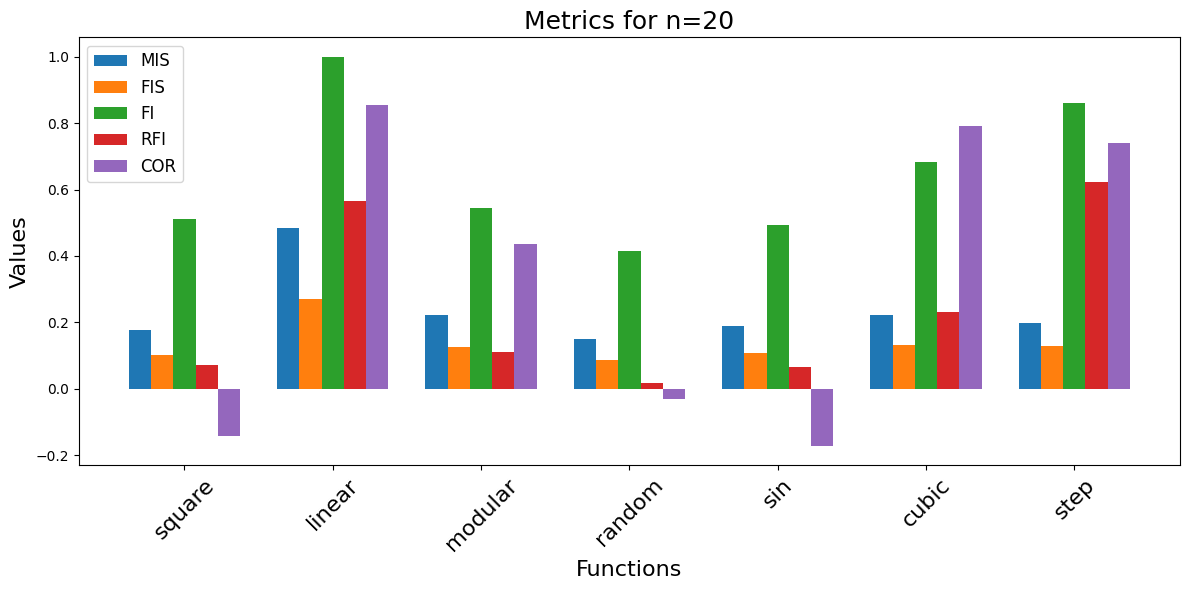
\includegraphics[width=0.8\textwidth]{images/n20eps03.png}
    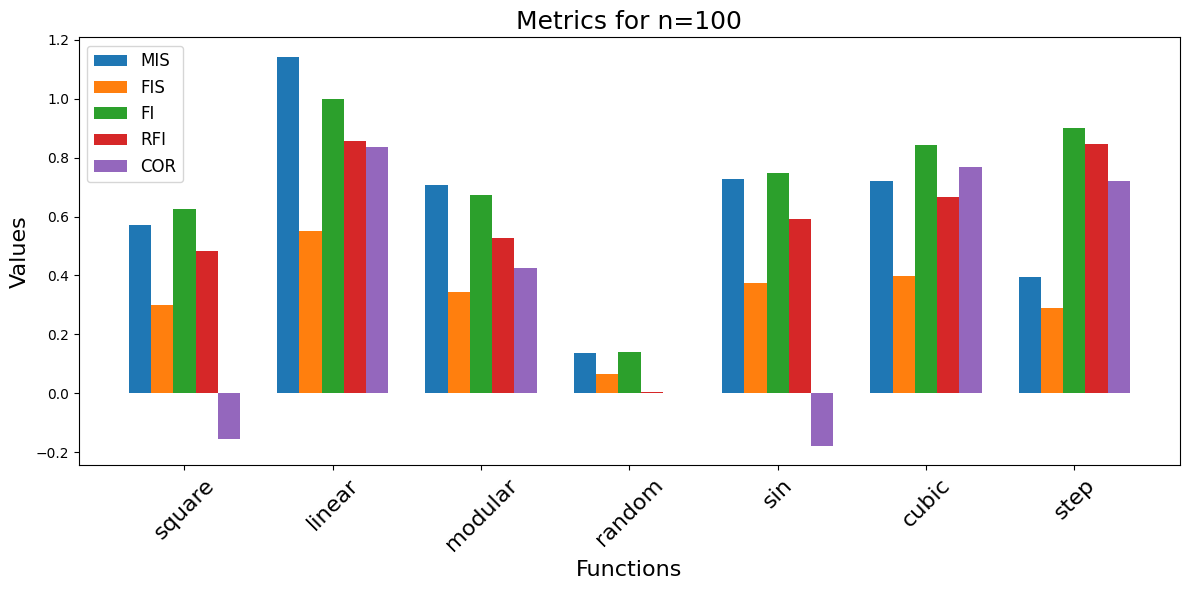
\includegraphics[width=0.8\textwidth]{images/n100eps03.png}
    \caption{Comparison of the Reliable Fraction of Information and the Smoothed Mutual Information on different functions for $n=20, n=100$. The metrics are abbreviated as follows: MIS - Mutual Information Smoothed, FIS - Fraction of Information Smoothed, FI - Fraction of Information (MLE), RFI - Reliable Fraction of Information, COR - Pearson Correlation}
    \label{fig:mi_comp}
\end{figure}

The results of the comparison are shown in \autoref{fig:mi_comp}. First of all, one can see that all metrics have troubles to some extent when the data is relatively sparse, i.e. $n=20$. The Smoothed Mutual Information assigns similar values to all but linear relationships. On the other hand, the Reliable Fraction of Information is able to distinguish between the random and other relationships, however, assigns very low values to sine, square and modular functions. The Fraction of Information (MLE) is not able to distinguish the random relationship at all as expected as it does not account for the bias. While the Pearson Correlation is able to distinguish the random relationship, but having troubles with non-linear types, also unsurprising.

When the number of samples is increased to $n=100$, one can see that all metrics can distinguish the random relationship from the others. However, few assign actual zero values to the random relationship. Furthermore, all metrics seem to prefer the linear and step function relationships. This is a crucial observation, since the main purpose of the metrics is to assign higher values to the relationships without implications of the underlying structure of the data. However, this observation becomes less relevant under not as sparse data $(n=100)$. 

This analysis gives some insight into the behavior of the mutual information estimators. However, it is not exhaustive and further more thorough analysis is needed to understand the behavior of the estimators in different scenarios. Moreover, some of the interpretations do not align with empirical results of Branch-and-Bound algorithms. For example as the Reliable Fraction of Information can way better distinguish the random relationship from the others, I would expect that the resulting Branch-and-Bound algorithm would have a lower false positive rate than one based on the Smoothed Mutual Information. Which is not the case in practice \citep{pennerath2020}.

\section{Markov Blankets and Top-k Dependencies}
Discovering the top-k dependencies between the features and the target variable is a task that is closely related to the problem of finding the Markov blanket of the target variable. The Markov blanket is a set of features that contains all the useful information about the target variable. In other words, the Markov blanket is a minimal set of features that can be used to predict the target variable. The problem of finding the Markov blanket is a well-known problem in machine learning \citep{tsamardinos2003}.

The most basic idea of finding the Markov blanket is Incremental Association Markov Blanket (IAMB) \citep{tsamardinos2003}. The algorithm starts with an empty set of features and iteratively adds features to the set if a certain heuristic value is greater than zero for the feature. This is a forward pass. After that, the algorithm performs a backward pass, which removes features from the set if a certain independence test shows that the feature is independent to the target variable. Theoretically, this algorithm is guaranteed to find the Markov blanket of the target variable. 

If one compares the IAMB algorithm with the Best-First Branch-and-Bound algorithm for the top-k dependencies problem, one can see that the ideas behind are quite similar. However, there are a few substantial differences. 

The first one is that the IAMB has a linear search space, that is it does not consider all possible subsets of features, but only a linear number of them testing them one by one. Here one can notice a deeper problem of the IAMB algorithm, as it does not consider all possible subsets of features, but only compares them one by one, one can construct a counterexample where the IAMB algorithm will not pick the optimal set of features. Consider the set of features $X = \{X_1, X_2\}$ and the target variable $Y$. Suppose that $Y=X_1 \oplus X_2$, where $\oplus$ is the XOR operation. Constructing a full truth table for this case, one can see that pairwise $X_1$ and $X_2$ are independent of $Y$. In particular if one considers heuristic based on the mutual information, it will be zero for both $I(X_1; Y)$ and $I(X_2; Y)$. However, combining the variables $X_1$ and $X_2$ together, one can see that they perfectly describe the target variable $Y$. Hence, the IAMB algorithm will not find the optimal set of features in this case. 

On the other hand, the Best-First Branch-and-Bound algorithm considers all possible subsets of features. However, this case is also not that trivial since the outcome of the algorithm depends on the branching and bounding functions. However, Branch-and-Bound algorithm clearly has a possibility to find the optimal set of features for this case, since it the branch function is able to generate the set $\{X_1, X_2\}$ and once it is generated, it will be immediately selected as part of the top-k dependencies. 

From this example one can conclude that the IAMB algorithm is not guaranteed to find the optimal set of features, and in general would be more prone to false negatives, since it only considers pairwise dependencies between the features and the target variable.

The second difference is in the absence of the backward pass in the Branch-and-Bound algorithm, as it is expected to take only the most optimal features. In this case, much dependence on the bounding function, if not chosen carefully, can lead to false positives, which will not be excluded later on. On the other hand, the IAMB is less prone to false positives, since it removes features that are independent of the target variable. This is one way of interpreting the backward pass and its results on the comparison with the Branch-and-Bound algorithm. However, much depends on the particular dataset as well as the particular choice of the bounding function and independence test in case of IAMB.



\section{Conclusion}
In this report, we discussed the topic of estimating the mutual information between the features and the target variable. We reviewed two approaches to this problem: the Reliable Fraction of Information and the Smoothed Mutual Information.

Furthermore, the practical usage of the metrics was discussed in the context of the top-k dependencies problem. The Branch-and-Bound algorithm is a practical solution to this problem, however, there is future work to be done in order to improve the efficiency of the algorithm.

In addition, we compared the mutual information estimators on some synthetic data. This simple analysis revealed some insights, however, a more thorough analysis is necessary which was not the point of this review. Furthermore, we developed connection to Markov blankets and the top-k dependencies problem and what differences there are between the IAMB algorithm and the Branch-and-Bound algorithm.


\bibliographystyle{apacite}	
\bibliography{references}


\appendix
\newpage
\section{Appendix}
\subsection{Visualization of the Functions}
\begin{figure}[h]
    \centering
    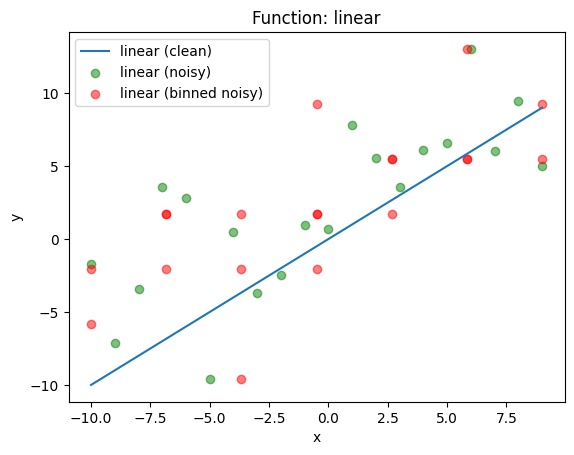
\includegraphics[width=0.4\textwidth]{images/linear20.png}
    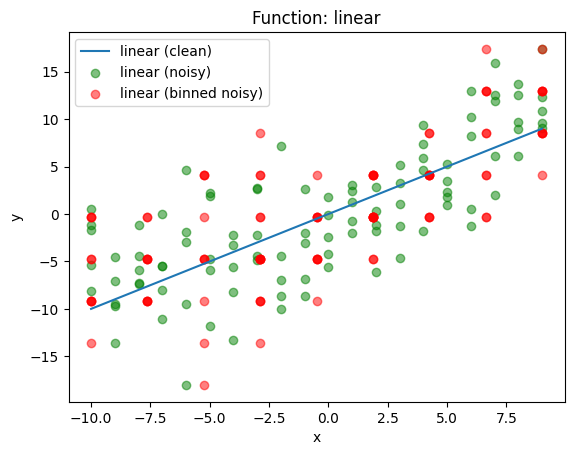
\includegraphics[width=0.4\textwidth]{images/linear100.png}
    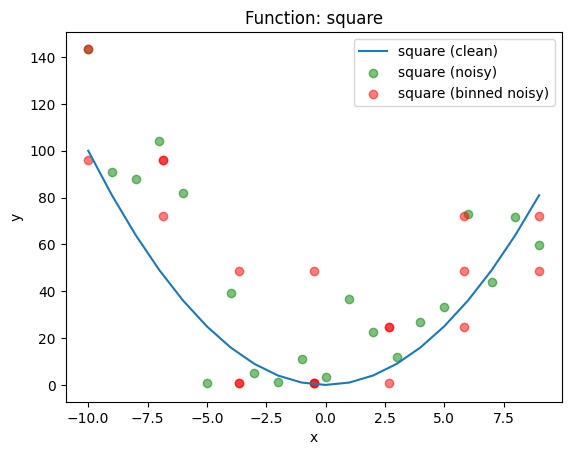
\includegraphics[width=0.4\textwidth]{images/quad20.png}
    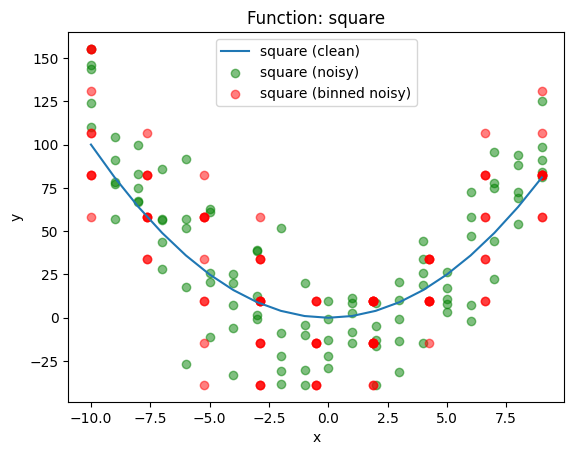
\includegraphics[width=0.4\textwidth]{images/quad100.png}
    \caption{Visualization of the linear and quadratic functions for $n=20$ and $n=100$. The noise is added such that $1-R^2=0.3$. The green scatter points are the points with added noise, while the red scatter points are the corresponding samples after binning.}
    \label{fig:funcs}
\end{figure}


\end{document}


